\subsection{Algorithm Testing}
Multiple different algorithms have been investigated for this report; standard evolution against n+n evolution, and local sensing against space aware sensing. These two factors combine to provide four statistical comparisons between algorithms:
\begin{enumerate}
  \item \verb|local-standard| vs \verb|local-n+n|
  \item \verb|space_aware-standard| vs \verb|space_aware-n+n|
  \item \verb|local-standard| vs \verb|space_aware-standard|
  \item \verb|local-n+n| vs \verb|space_aware-n+n|
\end{enumerate}
Each algorithm was ran 10 times with a population of 200 for 500 generations, an average of these runs was then computed to provide a fair representation of the performance of each algorithm. 

\subsubsection{standard evolution compared to n+n evolution}

As seen in figure \ref{1-2} comparing standard evolution to n+n for local collision sensing, while \verb|local-standard| was the prevailing algorithm after 500 generations, \verb|local-n+n| is consistently performs better from generation 0 until a crossover point at approximately 50 score. Performing a Mann-Whitney-U test for the two datasets at each generation gives an average of: 
$$
U = 107778.5, p = 0.00016
$$

Figure \ref{3-4} compares standard to n+n evolution for space aware collision sensing. As shown in the graph, n+n performed significantly better than standard evolution, though standard deviation was large. Standard evolution struggled to make any progress Throughout generations, with a consistently average score throughout generations of 0.

\begin{figure}[h]
  \centering
  \begin{minipage}{.5\textwidth}
    \centering
    \captionsetup{width=.8\linewidth}
    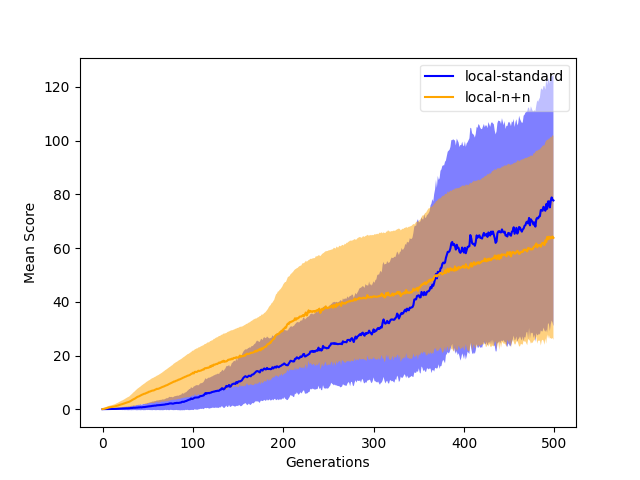
\includegraphics[width=1 \linewidth]{1-2}
    \caption{\texttt{local-standard} compared to \texttt{local-n+n} over 500 generations}
    \label{1-2}
  \end{minipage}%
  \begin{minipage}{.5\textwidth}
    \centering
    \captionsetup{width=.8\linewidth}
    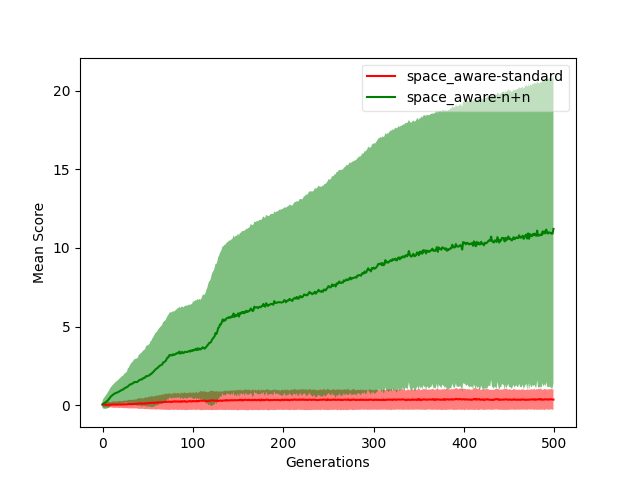
\includegraphics[width=1\linewidth]{3-4}
    \caption{\texttt{space\_aware-standard} compared to \texttt{space\_aware-n+n} over 500 generations}
    \label{3-4}
  \end{minipage}
\end{figure}

